\section{V.A. Lebesgue's proof of the case \texorpdfstring{\(q = 2\)}{q = 3}}

\begin{frame}
\frametitle{The case \texorpdfstring{\(q = 2\)}{q = 2}}

\begin{theorem}[V.A. Lebesgue, 1850]
The equation
\[
    x^p - y^2 = 1
\]
has no solutions in \(\integers^{*}\) for \(p \geq 2\).
\end{theorem}
\end{frame}

\begin{frame}
\frametitle{Lebesgue's proof of the case \texorpdfstring{\(q = 2\)}{q = 2}}

\begin{remark}
If \(p = 2\), the original equation becomes
\[
    (x - y)(x + y) = 1
\]
and the only solutions are \(\pm 1\) and \(0\). We may therefore assume that \(p\) is an \textbf{odd} prime number.
\end{remark}
\end{frame}

\begin{frame}
\frametitle{Lebesgue's proof of the case \texorpdfstring{\(q = 2\)}{q = 2}}

\begin{remark}
If \(2 \divides x\), then \(4 \divides x^p\) (since \(p > 2\)), whence
\begin{align*}
    y^2 + 1 &\equiv 0 \mod{4} \\
    \iff
    y^2 &\equiv -1 \mod{4}
\end{align*}
which has no solutions in \(\integers/4\integers\), so our initial assumption that \(2 \divides x\) cannot hold. Hence, \(x\) must be \textbf{odd} and \(y\) must be \textbf{even}.
\end{remark}
\end{frame}

\begin{frame}
\frametitle{Lebesgue's proof of the case \texorpdfstring{\(q = 2\)}{q = 2}}

With these remarks, the theorem becomes:
\begin{theorem}
The equation
\[
    x^p - y^2 = 1
\]
has no solutions in \(\integers^*\) for \(x\) odd, \(y\) even and \(p \geq 3\).
\end{theorem}
\end{frame}

\begin{frame}
\frametitle{Lebesgue's proof of the case \texorpdfstring{\(q = 2\)}{q = 2}}

Lebesgue's idea \cite{Lebesgue1850} was to factor the equation as
\[
    x^p = y^2 + 1 = (y + i)(y - i)
\]
and work in the ring of Gaussian integers \(\integers[i]\).
\end{frame}

\begin{frame}
\frametitle{The ring of Gaussian integers}

\begin{figure}
    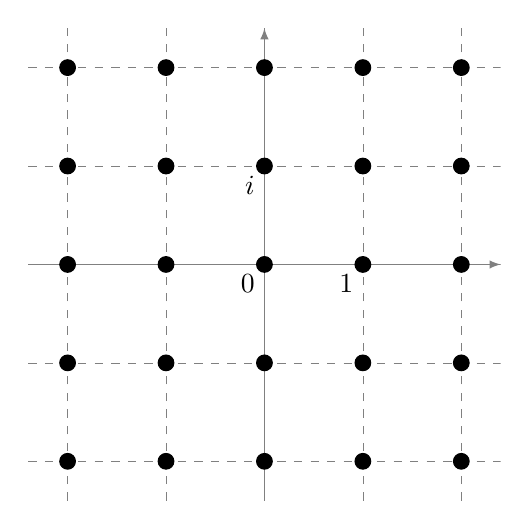
\begin{tikzpicture}
        \coordinate (XAxisMin) at (-3,0);
        \coordinate (XAxisMax) at (3,0);
        \coordinate (YAxisMin) at (0,-3);
        \coordinate (YAxisMax) at (0,3);
        \draw [thin, gray,-latex] (XAxisMin) -- (XAxisMax);
        \draw [thin, gray,-latex] (YAxisMin) -- (YAxisMax);
    
        \clip (-3,-3) rectangle (3cm,3cm);
    
        \pgftransformcm{1}{0}{0}{1}{\pgfpoint{0cm}{0cm}}

        \draw[style=help lines,dashed] (-3,-3) grid[step=1.25cm] (3,3);
        \foreach \x in {-2,-1,...,2}{
          \foreach \y in {-2,-1,...,2}{
            % Places a dot at those points
            \node[draw,circle,inner sep=2pt,fill] at (1.25*\x,1.25*\y) {};
          }
        }
        
        \node[below left] at (0, 0) {\(0\)};
        \node[below left] at (1.25, 0) {\(1\)};
        \node[below left] at (0, 1.25) {\(i\)};
    \end{tikzpicture}
    \caption*{The ring \(\integers[i]\)}
\end{figure}
\end{frame}

\begin{frame}
\frametitle{Lebesgue's proof of the case \texorpdfstring{\(q = 2\)}{q = 2}}

Since \(\integers[i]\) is an unique factorisation domain, the decomposition
\[
    x^p = y^2 + 1 = (y - i) (y + i)
\]
is unique up to units.
\end{frame}

\begin{frame}
\frametitle{Lebesgue's proof of the case \texorpdfstring{\(q = 2\)}{q = 2}}

\begin{proposition}
The elements \(y - i\) and \(y + i\) are coprime in \(\integers[i]\).
\end{proposition}

\begin{proof}
If \(\symfrak{p}\) is a prime in \(\integers[i]\) which divides both \(y - i\) and \(y + i\), it must divide \((y - i) + (y + i) = 2i\). Since \(i\) is a unit in \(\integers[i]\), we have \(\symfrak{p} \divides 2\). This shows that \(2 \divides x\), a contradiction.
\end{proof}
\end{frame}

\begin{frame}
\frametitle{Lebesgue's proof of the case \texorpdfstring{\(q = 2\)}{q = 2}}

This allows us to deduce that both \(y - i\) and \(y + i\) are \(p\)th powers in \(\integers[i]\), i.e.\
\begin{align*}
    y + i &= (u + i v)^p \\
    y - i &= (u - i v)^p
\end{align*}
for some \(u, v \in \integers\). \\[1em]
\end{frame}

\begin{frame}
\frametitle{Lebesgue's proof of the case \texorpdfstring{\(q = 2\)}{q = 2}}

Lebesgue proceeds by expanding out these \(p\)th powers using the binomial formula, compares their real and imaginary parts and then reaches a contradiction by comparing the greatest power of \(2\) which divides both sides. \\[1em]

In modern terms, he compared the \emph{\(2\)-adic valuation} of the two sides of the equality.
\end{frame}
